\chapter{Pilotstudie}
\label{sec:pilotstudie}

Dieses Kapitel prüft, ob das in dieser Arbeit entwickelte Erhebungsinstrument und der dazugehörige Fragebogen (\gls[noindex]{vgl} \cref{sec:entwicklung_app,sec:fragebogenentwicklung}) geeignet ist, Daten zu generieren, die sich für eine intersektional-quantitative Analyse nutzen lassen.

Als Testfall dient die folgende Überprüfungsfrage:
\begin{quote}
\emph{Wie beeinflussen räumliche Umgebungen das momentane Wohlbefinden intersektional positionierter Personen im Alltag?}
\end{quote}

Die Frage ist bewusst allgemein formuliert, da sie in dieser Pilotstudie nicht vollständig beantwortet, sondern methodisch erprobt wird. Ziel ist es zu untersuchen, ob die erhobenen Daten eine statistische Auswertung grundsätzlich zulassen und welche praktischen, technischen und konzeptionellen Herausforderungen dabei sichtbar werden.

Sämtlicher Code ist im \gls[noindex]{github}-Repository dieser Arbeit verfügbar.

\section{Stichprobe}

Die Datenerhebung fand im Rahmen der einführenden Exkursion Recht auf Stadt im ersten Studienjahr des Bachelorstudiengangs Geographie an der Universität Bern im Mai 2025 statt. Zu Beginn jedes der insgesamt vier Exkursionstage erfolgte eine Einladung zur freiwilligen Teilnahme an der Studie -- beim ersten Termin von mir persönlich, an den folgenden Terminen durch die Exkursionsleitenden. Für jede teilnehmende Person begann die Erhebungsphase mit einer einmaligen Baseline-Befragung und dauerte ab diesem Zeitpunkt sieben Tage.

\subsection*{Demographische Daten aus der Baseline Befragung}

Insgesamt wurden rund \num{80} Personen zur Teilnahme eingeladen. \num{24} davon schlossen mindestens die einmalige Baseline-Befragung vollständig ab und wurden in die Stichprobe aufgenommen. \num{8} begonnene, aber nicht abgeschlossene Baseline-Befragungen wurden ausgeschlossen. Ebenfalls ausgeschlossen wurden \num{6} während der Erhebungsphase begonnene, aber nicht abgeschlossene Momentaufnahmen. Die endgültige Stichprobe umfasst somit \num{24} Personen. \cref{tab:kreuztabelle_abs} zeigt die Verteilung von sozialem Geschlecht und Altersgruppe.

\begin{longtable}{lcccS}
    \caption{Kreuztabelle: Soziales Geschlecht und Altersgruppe (absolute Häufigkeiten)}
    \label{tab:kreuztabelle_abs}\\
    
    \toprule
    \textbf{Geschlecht} & 16--25 & 26--35 & Keine Angabe & \multicolumn{1}{c}{Gesamt} \\
    \midrule
    \endfirsthead
    
    \toprule
    \textbf{Geschlecht} & 16--25 & 26--35 & Keine Angabe & \multicolumn{1}{c}{Gesamt} \\
    \midrule
    \endhead
    
    \midrule
    \multicolumn{5}{r}{\textit{Fortsetzung auf der nächsten Seite}} \\
    \endfoot
    
    \bottomrule
    \endlastfoot
    
    Mann & 12 & 2 & 1 & 15 \\
    Frau &  8 & 1 & 0 &  9 \\
    \midrule
    \textbf{Gesamt} & 20 & 3 & 1 & 24 \\
    \end{longtable}
    
  

Die Mehrheit der Teilnehmenden verfügt über eine \emph{Matura oder ein gleichwertiges Abschlusszeugnis} (\num{22}; \SI{92}{\percent}), zwei Personen (\SI{8}{\percent}) besitzen einen Hochschulabschluss. Der überwiegende Teil ist als \emph{Student\genderstern in oder Schüler\genderstern in} erwerbstätig (\num{21}; \SI{88}{\percent}), drei Personen (\SI{12}{\percent}) sind angestellt. Die grosse Mehrheit wurde im gleichen Land geboren, in dem sie derzeit lebt (\num{16}; \SI{68}{\percent}), \num{7} Personen (\SI{28}{\percent}) nicht; eine Person (\SI{4}{\percent}) machte keine Angabe.  
Alle Personen gaben keine vorhandene Behinderung an (\num{24}; \SI{100}{\percent}).

Bezüglich der sexuellen Orientierung gaben \num{17} Personen (\SI{68}{\percent}) \emph{hetero} an, jeweils drei (\SI{12}{\percent}) \emph{homosexuell} oder \emph{bisexuell}, und eine Person (\SI{4}{\percent}) \emph{queer}. 

Beim gruppierten Äquivalenzeinkommen entfallen \num{8} Personen (\SI{32}{\percent}) auf die Kategorie \emph{Sehr niedrig}, \num{6} (\SI{24}{\percent}) machten keine Angabe, \num{5} (\SI{20}{\percent}) gehören zur Kategorie \emph{Hoch}, \num{4} (\SI{16}{\percent}) zu \emph{Niedrig} und \num{1} (\SI{4}{\percent}) zu \emph{Sehr hoch}.

Die hier gewählte Darstellung trennt die einzelnen Merkmale bewusst auf, um die Zusammensetzung der Stichprobe transparent zu machen. Methodisch betrachtet widerspricht diese Entzerrung jedoch einem intersektionalen Ansatz, da \glspl[noindex]{identitaetsachse} in isolierte Kategorien zerlegt werden. Die vollständige Übersicht über die Angaben aus der Baseline Befragung ist im \cref{app:appendix_demographics}.

\subsection*{Momentaufnahmen}

Insgesamt wurden \num{106} vollständig abgeschlossene Momentaufnahmen erhoben.  
Die Verteilung der Anzahl abgeschlossener Momentaufnahmen pro Person ist in \cref{fig:survey_counts} dargestellt.

Die Verteilungen der während der Momentaufnahmen angegebenen Tätigkeiten und Aufenthaltsortkategorien sind in \cref{fig:survey_activities} bzw. \cref{fig:survey_locations} dargestellt.  
Innenräume ($n = \num{54}; \SI{51}{\percent}$) und Aussenräume ($n = \num{52}; \SI{49}{\percent}$) waren nahezu gleich häufig vertreten.

Das soziale Umfeld variierte: Etwa ein Drittel der Momentaufnahmen wurde allein durchgeführt ($n = \num{37}; \SI{35}{\percent}$), ein weiteres Drittel in Gegenwart von Freund\genderstern innen ($n = \num{28}; \SI{26}{\percent}$). Weitere Angaben betrafen die Anwesenheit von Fremden ($n = \num{10}; \SI{9}{\percent}$), Kolleg\genderstern innen ($n = \num{8}; \SI{8}{\percent}$) oder Kombinationen dieser Gruppen (\gls[noindex]{vgl} \cref{app:people_table}).

\begin{figure}[h]
    \centering
    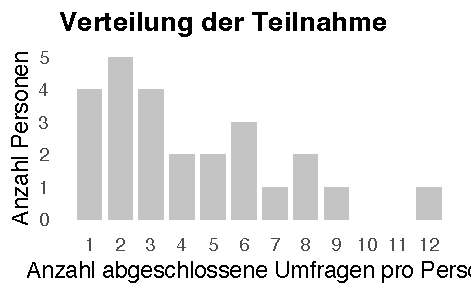
\includegraphics[width=8cm]{Analyse/Plots/survey_counts.pdf}
    \caption{Verteilung der Anzahl abgeschlossener Momentaufnahmen pro Person}
    \label{fig:survey_counts}
\end{figure}

\begin{figure}[h]
    \centering
    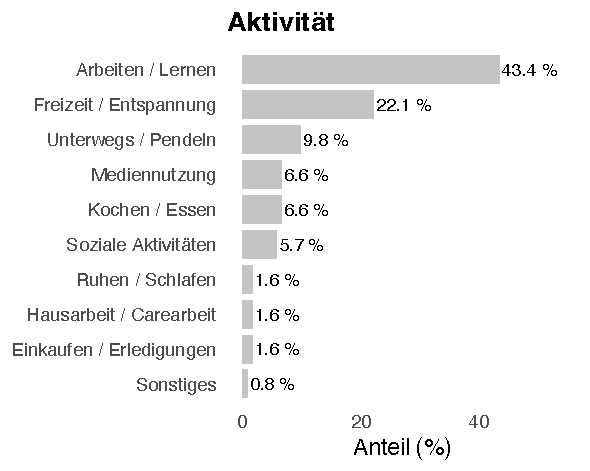
\includegraphics[width=10cm]{Analyse/Plots/cat_dist_activity.pdf}
    \caption{Tätigkeit während der Momentaufnahme}
    \label{fig:survey_activities}
\end{figure}

\begin{figure}[h]
    \centering
    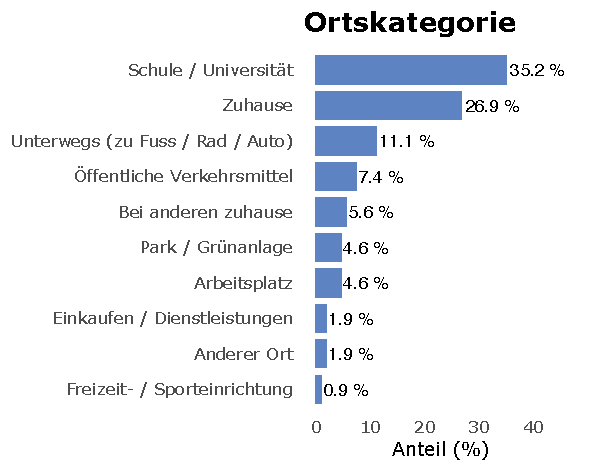
\includegraphics[width=10cm]{Analyse/Plots/cat_dist_location_category.pdf}
    \caption{Aufenthaltsortkategorie während der Momentaufnahme}
    \label{fig:survey_locations}
\end{figure}


\section{Quantitativ-intersektional analysieren -- Ein Widerspruch?}

Wie im theoretischen Rahmen zu Intersektionalität (\cref{sec:theoretischer_rahmen}) dargelegt, besteht eine grundlegende Spannung zwischen den theoretischen Ansprüchen intersektionaler Forschung und den Anforderungen quantitativer Analyseverfahren. Während Intersektionalität auf die komplexe, relationale und kontextabhängige Überlagerung sozialer Kategorien abzielt, verlangen statistische Modelle in der Regel klar definierte, operationalisierte Variablen. Damit einher geht die Gefahr, fluid-dynamische Identitäten in starre Kategorien zu übersetzen und deren soziale Konstruiertheit zu verschleiern \parencite{hancockWhenMultiplicationDoesnt2007, bowlegInvitedReflectionQuantifying2016}. Hinzu kommt, dass viele herkömmliche Verfahren additive oder eindimensionale Effekte modellieren, wodurch genau jene Interdependenzen und Wechselwirkungen nivelliert werden, die intersektionale Ansätze sichtbar machen wollen \parencite{scottIntersectionalityQuantitativeMethods2017}.

Diese methodische Spannung ist nicht nur ein technisches Problem, sondern berührt den Kern intersektionaler Forschung: Die Gefahr, sozial konstruierte Kategorien wie feste, unveränderliche Eigenschaften zu behandeln, steht im Widerspruch zu ihrem theoretischen Verständnis als historisch, räumlich und sozial wandelbare Konstrukte. Jede quantitative Operationalisierung muss daher reflexiv mit diesen Grenzen umgehen und das Risiko methodischer Vereinfachungen offenlegen \parencite{rodo-de-zarateDevelopingGeographiesIntersectionality2014, websterCenteringSocialtechnicalRelations2021}.

Vor diesem Hintergrund wird in dieser Pilotanalyse ein \acrfull{maihda}\footnote{In der Literatur finden sich sowohl die Bezeichnungen \emph{\acrfull{maihda}} als auch \emph{\acrfull{i-maihda}} \parencite{evansTutorialConductingIntersectional2024}. Beide Begriffe beziehen sich auf das gleiche statistische Verfahren; die Bezeichnung mit vorangestelltem „I“ hebt den Bezug zu intersektionaler Theorie explizit hervor. In dieser Arbeit wird \emph{\gls{i-maihda}} verwendet, um diesen theoretischen Rahmen klar zu signalisieren.} eingesetzt. \gls{i-maihda} ist ein flexibles, mehrstufiges Analysemodell, das Daten in Gruppen („\glspl{stratum}“) verschachtelt, die sich aus der Kombination mehrerer sozialer Merkmale ergeben. Jede Person gehört genau zu einem solchen sozialen \gls{stratum}. Innerhalb eines sozialen \gls{stratum} können sich die Werte der untersuchten Variablen (\gls[noindex]{zb} Wohlbefinden) zwischen Personen unterscheiden, während sich gleichzeitig Unterschiede zwischen den sozialen \glspl{stratum} selbst zeigen.

Aus statistischer Sicht handelt es sich um ein hierarchisches Modell, das mindestens zwei Ebenen umfasst: \textit{Level 1} sind die einzelnen Beobachtungen, \textit{Level 2} die sozialen \glspl{stratum}. \gls{i-maihda} schätzt, wie sich die Gesamtvarianz -- also die Streuung der Messwerte im gesamten Datensatz -- auf unterschiedliche Ebenen verteilt. Dabei wird getrennt zwischen Varianz, die zwischen den sozialen \glspl{stratum} liegt, und Varianz, die innerhalb der sozialen \glspl{stratum} entsteht. Diese Zerlegung erlaubt es zu erkennen, in welchem Ausmass die Kombination sozialer Merkmale systematische Unterschiede im Outcome erklärt und wie viel der Unterschiede auf individuelle oder situative Faktoren zurückzuführen ist. In grossen Datensätzen ermöglicht dieser Ansatz die Modellierung komplexer \glspl{stratum} mit zahlreichen kombinierten Merkmalen, da pro sozielem \gls{stratum} genügend Beobachtungen vorliegen, um stabile und präzise Schätzungen zu erhalten.

Der zentrale Vorteil von \gls{i-maihda} gegenüber klassischen Regressionsmodellen liegt darin, dass nicht nur einzelne Haupteffekte und ausgewählte Interaktionsterme berücksichtigt werden, sondern jede Merkmalskombination als eigenständige Analyseeinheit behandelt wird \parencite{hancockWhenMultiplicationDoesnt2007, bowlegInvitedReflectionQuantifying2016}. Zudem ermöglicht \gls{i-maihda} die Berechnung der sogenannten „diskriminatorischen Genauigkeit“ -- ein Mass dafür, wie trennscharf die gewählten sozialen \glspl{stratum} das Outcome im jeweiligen Kontext erklären \parencite{evansTutorialConductingIntersectional2024}.

Trotz dieser Stärken ist \gls{i-maihda} kein ursprünglich intersektionales Verfahren. Es ist aus der epidemiologischen Mehrebenenanalyse hervorgegangen und wurde nicht primär entwickelt, um intersektionale Theorien oder Machtverhältnisse theoretisch zu adressieren. Seine intersektionale Anschlussfähigkeit entsteht erst durch eine bewusste, theoriegeleitete Auswahl der Merkmale, eine reflektierte Modellierung und die Einbettung der Ergebnisse in einen sozialen und politischen Kontext \parencite{grossModellingIntersectionalityQuantitative2023}. In diesem Sinne kann \gls{i-maihda} helfen, die eingangs skizzierte Spannung zwischen theoretischem Anspruch und quantitativer Operationalisierung zu verringern -- sie jedoch nicht vollständig auflösen.

\section{Versuch einer Analyse}

Ziel dieser Pilotanalyse ist es, zu prüfen, ob und in welchem Ausmass sich Unterschiede im situativen Wohlbefinden durch die Kombination mehrerer sozialer \glspl{stratum} und durch situative Kontextfaktoren erklären lassen. Dabei wird ein mehrstufiges Analyseverfahren eingesetzt, das die Messwerte auf verschiedenen Ebenen der Datenhierarchie modelliert. Da die Datengrundlage klein und unbalanciert ist -- viele \glspl{stratum} enthalten nur eine Person und die Zahl der Wiederholungsmessungen pro Person ist gering -- dienen die folgenden Schritte primär der methodischen Illustration und nicht der inhaltlich belastbaren Beantwortung der Forschungsfrage.

Als abhängige Variable wird ein \emph{Wohlbefindensindex} verwendet, der aus fünf Einzelfragen gebildet wurde: \emph{Generelles Wohlbefinden}, \emph{Zufriedenheit}, \emph{Anspannung}, \emph{Energie} und \emph{Zugehörigkeit} (\gls{vgl} \cref{tab:moments}). Alle Items sind auf einen Wertebereich von $0$ bis $1$ skaliert, wobei höhere Werte stets ein positiveres Befinden darstellen. Durch die anschliessende Aggregation mittels des geometrischen Mittels wird vermieden, dass ein sehr hoher Wert in einer Dimension einen niedrigen Wert in einer anderen vollständig ausgleichen kann; zugleich wird der Einfluss einzelner Ausreisser reduziert.

Die zeitinvarianten erklärenden Variablen sind die vier Achsen \emph{\gls[noindex]{gender}}, \emph{Altersgruppe}, \emph{sexuelle Orientierung} und \emph{Äquivalenzeinkommensgruppe} (\gls{vgl} \cref{tab:soziodemografie_gesamt}). Die eindeutige Kombination dieser Merkmale definiert ein soziales \gls{stratum}. Damit gehört jede Person genau zu einem solchen \gls{stratum}.

Die zeitvariablen Kontextmerkmale beziehen sich auf die jeweilige Situation der Momentaufnahme und umfassen Aufenthaltsort (Innen- oder Aussenraum, spezifische Ortskategorie), Anwesenheit und Art der Beziehung zu anderen Personen, Hauptaktivität, Mehrheitsvergleich sowie vier metrische Bewertungen der Umgebung: wahrgenommene Lautstärke, sichtbare Natur, Lebhaftigkeit und empfundene Angenehmheit (\gls{vgl} \cref{tab:moments}).

Zur Modellierung werden kategoriale Variablen als Dummy-Variablen kodiert, wobei jeweils eine Referenzkategorie entfällt, um die statistische Identifizierbarkeit sicherzustellen. Die vier metrischen Umweltbewertungen werden \emph{person-mean}-zentriert, indem von jeder Beobachtung der individuelle Durchschnittswert der jeweiligen Person abgezogen wird. Ein positiver Wert zeigt an, dass eine Situation lauter, naturreicher, lebhafter oder angenehmer erlebt wird als für diese Person gewöhnlich. Dieses Vorgehen trennt kurzfristige Schwankungen innerhalb einer Person von stabilen Unterschieden zwischen Personen.

\subsection*{Modellbildung}

Das erste Modell ($M0_{3L}$) dient dazu, die Gesamtvarianz des Wohlbefindens auf die verschiedenen Ebenen zu zerlegen. Die Ebenen sind:

\begin{enumerate}
    \item \textbf{Level~1:} einzelne Momentaufnahmen,
    \item \textbf{Level~2:} Personen,
    \item \textbf{Level~3:} soziale \glspl{stratum}.
\end{enumerate}

\begin{longtable}{llll ccc}
    \caption{Übersicht über soziale \glspl[noindex]{stratum}}\label{tab:strata-uebersicht}\\
    \toprule
    Geschl. & Alter & Sex. Orient. & Äquiv.-Eink. & Pers. & Befr. & Befr./Pers.\\
    \midrule
    \endfirsthead
    
    \multicolumn{7}{c}{{Tabelle \thetable{} -- Fortsetzung}} \\
    \toprule
    Geschl. & Alter & Sex. Orient. & Äquiv.-Eink. & Pers. & Befr. & Befr./Pers.\\
    \midrule
    \endhead
    
    \midrule
    \multicolumn{7}{r}{Fortsetzung auf der nächsten Seite}\\
    \endfoot
    
    \bottomrule
    \endlastfoot
    
    weiblich    & 16 -- 25    & heterosexuell & Hoch           & 3 & 13 & 4.33 \\
    männlich    & 16 -- 25    & heterosexuell & Sehr niedrig   & 3 &  9 & 3.00 \\
    männlich    & 16 -- 25    & heterosexuell & \textemdash    & 2 &  9 & 4.50 \\
    weiblich    & 16 -- 25    & heterosexuell & \textemdash    & 2 &  8 & 4.00 \\
    weiblich    & 16 -- 25    & bisexuell     & \textemdash    & 1 & 12 & 12.00\\
    männlich    & 16 -- 25    & heterosexuell & Sehr hoch      & 1 &  9 & 9.00 \\
    männlich    & 16 -- 25    & heterosexuell & Niedrig        & 1 &  8 & 8.00 \\
    männlich    & 16 -- 25    & homosexuell   & Niedrig        & 1 &  7 & 7.00 \\
    weiblich    & 16 -- 25    & heterosexuell & Sehr niedrig   & 1 &  6 & 6.00 \\
    weiblich    & 26 -- 35    & heterosexuell & Sehr niedrig   & 1 &  5 & 5.00 \\
    männlich    & 26 -- 35    & heterosexuell & Sehr hoch      & 1 &  4 & 4.00 \\
    männlich    & 16 -- 25    & homosexuell   & Hoch           & 1 &  3 & 3.00 \\
    männlich    & 16 -- 25    & heterosexuell & Hoch           & 1 &  3 & 3.00 \\
    männlich    & 16 -- 25    & homosexuell   & \textemdash    & 1 &  3 & 3.00 \\
    männlich    & 16 -- 25    & bisexuell     & Sehr niedrig   & 1 &  2 & 2.00 \\
    weiblich    & 16 -- 25    & queer         & Sehr niedrig   & 1 &  2 & 2.00 \\
    \textemdash & \textemdash & \textemdash   & \textemdash    & 1 &  2 & 2.00 \\
    männlich    & 26 -- 35    & bisexuell     & Sehr niedrig   & 1 &  1 & 1.00 \\
    
\end{longtable}

Die Schätzung ergibt, dass rund \SI{8.9}{\percent} der Gesamtvarianz zwischen den \glspl{stratum} liegt, während auf der Personenebene keine eigenständige Varianz feststellbar ist. Mit anderen Worten: Innerhalb desselben \glspl{stratum} unterscheiden sich die mittleren Wohlbefindenswerte der einzelnen Personen in diesen Daten nicht systematisch. Der Grossteil der Varianz ($\approx$\SI{91.1}{\percent}) entfällt auf kurzfristige Schwankungen zwischen verschiedenen Momentaufnahmen derselben Person.

Diese fehlende Varianz auf der Personenebene ist eine direkte Folge der Datenstruktur: Viele \glspl{stratum} bestehen nur aus einer einzelnen Person, und auch bei den übrigen \glspl{stratum} liegt nur eine geringe Zahl an Wiederholungsmessungen pro Person vor. Unter diesen Bedingungen kann das Modell keine stabilen Unterschiede zwischen Personen desselben \gls{stratum} identifizieren. Eine dreistufige Modellierung ist daher hier nicht sinnvoll; die folgenden Schritte basieren auf einer reduzierten zweistufigen Struktur:

\begin{itemize}
    \item \textbf{Level~1:} Momentaufnahmen,
    \item \textbf{Level~2:} \glspl{stratum}.
\end{itemize}

Auch das zweistufige Nullmodell $(M0_{2L})$ ergibt für die sozialen \glspl{stratum} einen \gls{icc} von $\approx$\SI{8.9}{\percent}. Damit lassen sich knapp neun Prozent der Unterschiede im situativen Wohlbefinden auf systematische Differenzen zwischen den sozialen \glspl{stratum} zurückführen.

Im nächsten Schritt $(M1_{2L})$ werden die vier Achsen (\gls[noindex]{gender}, Altersgruppe, sexuelle Orientierung, Äquivalenzeinkommen) als additive Haupteffekte aufgenommen, um den durch Einzeleffekte erklärbaren Anteil dieser Unterschiede zu bestimmen -- ohne Wechselwirkungen zu berücksichtigen. Dieses bewusste \enquote{Auseinanderlegen} verdeutlicht die Spannung zwischen intersektionaler Theorie und quantitativer Analyse: Um den spezifischen Effekt einer Merkmalskombination zu isolieren, werden zunächst die erwarteten Einzeleffekte herausgerechnet. Das verbleibende Mass wird als \emph{intersektionaler Überschuss} bezeichnet.

In diesem Modell sinkt die geschätzte Varianz zwischen den sozialen \glspl{stratum} von \num{0.003024} auf \num{0.001110}, was einer \gls{pev} von rund \SI{63}{\percent} entspricht. Somit lassen sich etwa zwei Drittel der gruppenbezogenen Unterschiede durch die additiven Effekte der vier Achsen erklären; der verbleibende Anteil von rund einem Drittel beruht ausschliesslich auf deren spezifischer Kombination und stellt den intersektionalen Überschuss dar.

Im dritten Modell $(M2_{2L})$ werden zusätzlich die situativen Kontextvariablen aufgenommen. Die geschätzte Varianz zwischen den sozialen \glspl{stratum} sinkt dadurch nahezu auf Null, und auch die verbleibende Restvarianz reduziert sich deutlich. Relativ zum Nullmodell entspricht dies einer erklärten zwischenstratalen Varianz von etwa \SI{99.9}{\percent} sowie einer erklärten Restvarianz von etwa \SI{99.3}{\percent}. Damit lassen sich die Unterschiede im Wohlbefinden zwischen den sozialen \glspl{stratum} in dieser Stichprobe nahezu vollständig durch die Kombination aus Einzelachsen und situativen Kontextfaktoren erklären. Aufgrund der kleinen und unbalancierten Stichprobe ist dieses Ergebnis jedoch mit Vorsicht zu interpretieren.


\subsection*{Analyse variierender Umwelteinflüsse zwischen sozialen Strata}

Die Forschungsfrage dieses Kapitels zielt darauf, zu verstehen, inwieweit sich situative Umweltfaktoren unterschiedlich auf das Wohlbefinden verschiedener sozialer \glspl{stratum} auswirken. Während die bisherigen Modelle lediglich Mittelwertsunterschiede zwischen den \glspl{stratum} abbildeten (\emph{Random Intercepts}), wird dieser Schritt um \emph{Random Slopes} erweitert: Dadurch lässt sich modellieren, ob und wie stark sich die Wirkung einzelner Kontextfaktoren systematisch zwischen den sozialen \glspl{stratum} unterscheidet.

Methodisch eröffnet dieser Ansatz die Möglichkeit, \gls[noindex]{ema}- und \gls[noindex]{gema}-Daten so auszuwerten, dass nicht nur konstante Gruppenunterschiede, sondern auch unterschiedliche Sensitivitäten gegenüber situativen Einflüssen sichtbar werden. In dieser Pilotanalyse dient er der Illustration des methodischen Potenzials; inhaltliche Schlussfolgerungen sind aufgrund der kleinen und unbalancierten Stichprobe nicht möglich.

Für jede der vier metrischen Umweltbewertungen (\emph{Lautstärke}, \emph{sichtbare Natur}, \emph{Lebhaftigkeit} und \emph{empfundende Angenehmheit}) wurde ein separates Mehrebenenmodell mit zufälligen Steigungen geschätzt. Die Umweltvariablen wurden vorab \emph{person-mean}-zentriert und standardisiert, sodass die Koeffizienten als Veränderung des Wohlbefindens pro Anstieg um eine Standardabweichung gegenüber dem individuellen Mittelwert interpretiert werden können. Jedes Modell enthielt die vier sozialen Achsen als feste Effekte, während für die jeweilige Umweltvariable eine variierende Steigung (\emph{Random Slope}) pro \gls{stratum} geschätzt wurde. Aus den Modellen wurden stratum-spezifische Steigungen mit 95\%-Konfidenzintervallen extrahiert und in Tabelle~\ref{tab:effekte-pro-stratum} zusammengeführt.

\begin{ThreePartTable}
    \begin{TableNotes}[flushleft]
        \item $\Delta$ Wohlbefindensindex pro Anstieg der erklärenden Variable um eine Standardabweichung.
        \item \textbf{Fett} = Effekt ist statistisch signifikant (95\%-Konfidenzintervall schliesst den Wert 0 aus).
        \item (\textemdash = unbekannt)
    \end{TableNotes}
      
    \begin{longtable}{llllr rrrr}
        \caption{Effekte pro Stratum} 
        \label{tab:effekte-pro-stratum} \\
        \toprule
        Geschl. & Alter & Sex. Orient. & Äquiv.-Eink. & Befr. & Lärm & Natur & Lebhaftigkeit & Angenehmkeit \\
        \midrule
        \endfirsthead
        
        \multicolumn{9}{c}{{\bfseries Tabelle \thetable\ -- Fortsetzung}} \\
        \toprule
        Geschl. & Alter & Sex. Orient. & Äquiv.-Eink. & Befr. & Lärm & Natur & Lebhaftigkeit & Angenehmkeit \\
        \midrule
        \endhead
        
        \midrule
        \multicolumn{9}{r}{{Fortsetzung auf der nächsten Seite}} \\
        \endfoot
        
        \bottomrule
        \insertTableNotes
        \endlastfoot
        
        Frau & 16 -- 25 & heterosexuell & hoch         & 13 & \textbf{0.04} & 0.04          & 0.04          & 0.04          \\
        Frau & 16 -- 25 & bisexuell     & ---          & 12 & \textbf{0.04} & 0.05          & \textbf{0.07} & \textbf{0.07} \\
        Mann & 16 -- 25 & heterosexuell & ---          &  9 & \textbf{0.05} & \textbf{0.07} & 0.06          & 0.05          \\
        Mann & 16 -- 25 & heterosexuell & sehr hoch    &  9 & \textbf{0.04} & 0.01          & 0.01          & 0.03          \\
        Mann & 16 -- 25 & heterosexuell & sehr niedrig &  9 & \textbf{0.04} & \textbf{0.07} & 0.03          & 0.03          \\
        Mann & 16 -- 25 & heterosexuell & niedrig      &  8 & \textbf{0.04} & 0.03          & 0.00          & 0.02          \\
        Frau & 16 -- 25 & heterosexuell & ---          &  8 & \textbf{0.04} & 0.02          & 0.04          & 0.03          \\
        Mann & 16 -- 25 & homosexuell   & niedrig      &  7 & \textbf{0.05} & 0.07          & 0.05          & 0.05          \\
        Frau & 16 -- 25 & heterosexuell & sehr niedrig &  6 & \textbf{0.04} & 0.05          & 0.04          & 0.04          \\
        Frau & 26 -- 35 & heterosexuell & sehr niedrig &  5 & \textbf{0.04} & 0.04          & 0.03          & 0.04          \\
        Mann & 26 -- 35 & heterosexuell & sehr hoch    &  4 & \textbf{0.04} & 0.05          & 0.04          & 0.05          \\
        Mann & 16 -- 25 & homosexuell   & hoch         &  3 & \textbf{0.04} & 0.02          & 0.02          & 0.02          \\
        Mann & 16 -- 25 & heterosexuell & hoch         &  3 & \textbf{0.04} & 0.04          & 0.03          & 0.03          \\
        Mann & 16 -- 25 & homosexuell   & ---          &  3 & \textbf{0.04} & \textbf{0.07} & 0.03          & 0.02          \\
        Mann & 16 -- 25 & bisexuell     & sehr niedrig &  2 & \textbf{0.04} & 0.03          & 0.02          & 0.02          \\
        Frau & 16 -- 25 & queer         & sehr niedrig &  2 & \textbf{0.04} & 0.04          & 0.03          & 0.04          \\
    
    \end{longtable}
\end{ThreePartTable}

Einzelne Effektschätzungen waren statistisch signifikant (95\%-Konfidenzintervall schliesst 0 aus). Angesichts der geringen Fallzahlen pro Stratum und der unbalancierten Stichprobe sind diese Resultate jedoch nicht inhaltlich belastbar. Die Auswertung ist hier vor allem als Demonstration zu verstehen, wie heterogene Umwelteffekte entlang sozialer \glspl{stratum} modelliert und dargestellt werden können.

\subsection*{Methodische Beobachtungen und Implikationen}

Die Ergebnisse zeigen, dass sich mit den hier erhobenen \gls[noindex]{ema}- und \gls[noindex]{gema}-Daten grundsätzlich auch stratum-spezifische Umwelteffekte modellieren lassen. Die Umsetzung der \emph{Random-Slopes}-Modelle verlief technisch problemlos; die Modellschätzungen lieferten für jedes \gls{stratum} interpretierbare Effektkoeffizienten und Konfidenzintervalle. 

Gleichzeitig verdeutlicht die Analyse die hohen Anforderungen an die Datengrundlage: Die geringe Fallzahl pro \gls{stratum} führt zu breiten Konfidenzintervallen und erschwert die Trennung systematischer Unterschiede von zufälligen Schwankungen. Die unbalancierte Stichprobenstruktur bewirkt zudem, dass einige Strata vollständig von einzelnen Personen repräsentiert werden, wodurch Schätzungen stark durch individuelle Ausprägungen beeinflusst werden können. 

Die grossen Varianzanteile auf der Ebene der Momentaufnahmen deuten darauf hin, dass kurzfristige, situative Schwankungen einen erheblichen Einfluss auf das Wohlbefinden haben können -- unabhängig von stabilen Gruppenunterschieden. Methodisch unterstreicht dies den Mehrwert von \gls[noindex]{ema}- und \gls[noindex]{gema}-Designs, die solche intraindividuellen Veränderungen erfassen. 

Diese Beobachtungen legen nahe, dass das Verfahren für grössere, stärker ausbalancierte Datensätze geeignet ist, um vergleichbare Forschungsfragen belastbar zu beantworten. In der vorliegenden Pilotstudie dient es vor allem als Machbarkeitsnachweis und zur Identifikation von Herausforderungen, die bei einer weiteren Untersuchung gezielt adressiert werden können.

Darüber hinaus wurde in der Pilotanalyse bewusst darauf verzichtet, die tatsächlichen Standortdaten in die Modellierung einzubeziehen. Angesichts der kleinen Stichprobe hätte dies nur einen geringen inhaltlichen Mehrwert gebracht und potenziell Rückschlüsse auf \gls{bspw} den Wohnort einzelner Teilnehmenden ermöglicht. Sämtliche Standortdaten wurden vor der Veröffentlichung aus dem Datensatz entfernt. Für künftige Erhebungen mit grösserer Fallzahl bietet sich jedoch die Verknüpfung mit hochaufgelösten Kontextinformationen an, beispielsweise mit lokalen Hitzedaten \parencite[siehe][]{burgerModellingSpatialPattern2021} oder präziseren Geofences, um spezifische räumliche Kontexte gezielt zu analysieren.

